\documentclass[10pt]{article}
\usepackage[english]{babel}
\usepackage[latin1]{inputenc}
\usepackage{subfigure}
\usepackage{epsfig}
\usepackage{amsmath,amssymb}
\usepackage{pdfpages}
\parindent 0mm
\textwidth 16cm
\textheight 23cm
\oddsidemargin 0cm
\evensidemargin 0cm
\topmargin -10mm
\newcommand{\vect}[1]{{\bf{#1}}}
\newcommand{\svect}[1]{\boldsymbol{#1}}
\newcommand{\matr}[1]{\boldsymbol{#1}}

\renewcommand{\vec}[1]{\mathbf{#1}}
\newcommand{\set}[1]{\mathcal{#1}}
\newcommand{\C}{\set{C}}
\newcommand{\E}{\mathcal{E}}
\newcommand{\I}{\vec{I}}
\renewcommand{\L}{\mathcal{L}}
\newcommand{\N}{\mathrm{I \negmedspace N}}
\newcommand{\R}{\mathrm{I \negmedspace R}}
\newcommand{\V}{\set{V}}
\newcommand{\W}{\vec{W}}
\newcommand{\X}{\set{X}}
\newcommand{\e}{\vec{e}}
%\newcommand{\f}[1]{\mathrm{#1}} %funktio
\newcommand{\h}{\vec{h}}
\newcommand{\m}{\vec{m}}
\newcommand{\mub}{\boldsymbol{\mu}}
\newcommand{\n}{\vec{n}}
\renewcommand{\t}{\vec{t}}
\renewcommand{\u}{\vec{u}}
\renewcommand{\v}{\vec{v}}
\newcommand{\w}{\vec{w}}
\newcommand{\x}{\vec{x}}
\newcommand{\y}{\vec{y}}
\newcommand{\Y}{\vec{Y}}
\newcommand{\z}{\vec{z}}
\newcommand{\argmin}{\operatornamewithlimits{argmin}}
\newcommand{\argmax}{\operatornamewithlimits{argmax}}
\newcommand{\bSigma}{\boldsymbol{\Sigma}}



\begin{document}
\pagestyle{empty}
\begin{Large}
\begin{bf} 
T-61.5130 Machine Learning and Neural Networks\\ 
\end{bf}
\end{Large}
Karhunen, Hao Tele\\
\\
\begin{large}
\begin{bf}
Exercise 9,  2.12.2011\\Model answer
\end{bf}
\end{large}
\begin{enumerate}

\item Consider a random input vector $\mathbf{X}$ made up of two component vectors,
 $\mathbf{X} = [\mathbf{X}_1,\mathbf{X}_2]^T$. Assume that you would like to represent the
 central dependencies between $\mathbf{X}_1$ and $\mathbf{X}_2$ with a  simple
 model. How would you do that? (Hint: Consider linear combinations.)

---------------------------------------------------------------------------------------------

 If we are not interested in the dependencies inside the groups
  $\vec{X}_1$ or $\vec{X}_2$ but are interested only on dependecies
  between these groups, we can use canonical correlation analysis (CCA).  It
  means that we try to find projections from $\vec{X}_1$ and
  $\vec{X}_2$ which would be as correlated as possible. CCA uses only
  second-order statistics; for Gaussian variables this
  is sufficient but CCA can also be used for
  non-Gaussian variables. For a tutorial on CCA, see,
  e.g., the one by Magnus Borga available
  at http://people.imt.liu.se/$\sim$magnus/cca/ . The following is
  partly based on the information in that tutorial.

  The correlation coefficient between zero mean random variables $a$
  and $b$ is defined to be $\rho_{ab} =
  E\{ab\}/\sqrt{E\{a^2\}E\{b^2\}}$.  We have projections $a_i = \u_i^T
  \x_1$ and $b_i = \v_i^T \x_2$ and we would like to maximise the
  correlations between $a_i$ and $b_i$. We restrict the solutions to be
  uncorrelated for different $i$: $E\{a_i a_j\} = E\{b_i b_j\} = E\{a_i b_j\} = 0$
  for $i \neq j$.

  For the $i$th projections we have
  \begin{align*}\nonumber
  \rho_{a_i b_i}
  = \frac{E\{\u_i^T \x_1 \x_2^T \v_i\}}{\sqrt{E\{\u_i^T \x_1\x_1^T\u_i\} E\{\v_i^T \x_2\x_2^T\v_i\}}}
  &= \frac{\u_i^T E\{\x_1 \x_2^T\} \v_i}{\sqrt{\u_i^T E\{\x_1\x_1^T\}\u_i \v_i^T E\{\x_2\x_2^T\}\v_i}} \\
  &= \frac{\u_i^T \boldsymbol{\Sigma}_{12} \v_i}{\sqrt{\u_i^T \boldsymbol{\Sigma}_1\u_i \v_i^T \boldsymbol{\Sigma}_2\v_i}} \;.
  \end{align*}

  It can be shown that the maximization corresponds to solving either one
  of the following eigenvalue equations:
  $$
  \bSigma_1^{-1}\bSigma_{12}\bSigma_2^{-1}\bSigma_{12}^T\u_i=\rho^2_{a_i b_i}\u_i
  $$
  $$
  \bSigma_2^{-1}\bSigma_{12}^T\bSigma_1^{-1}\bSigma_{12}\v_i=\rho^2_{a_i b_i}\v_i \;.
  $$


  \paragraph{Connection to singular value decomposition.}
  Canonical correlations are invariant to affine transformations (for example,
  if a transformation $\mathbf{A}$ is used for $\x_1$, just set $\hat \u_i=\mathbf{A}^{-1}\u_i$).
  Therefore, to simplify the situation, suppose that $\vec{X}_1$ and $\vec{X}_2$ have been whitened
  (see problem 3 for the precise transformations needed).
  Then $\bSigma_1=\mathbf{I}$ and $\bSigma_2=\mathbf{I}$. (Note that $\vec{X}_1$ and $\vec{X}_2$
  can have different dimensionalities, so the two identity matrices can be of different sizes.)
  The eigenvalue equations then become
  \begin{equation}\label{eq:temp1}
  \bSigma_{12}\bSigma_{12}^T\u_i=\rho^2_{a_i b_i}\u_i\;,\;
  \bSigma_{12}^T\bSigma_{12}\v_i=\rho^2_{a_i b_i}\v_i \;.
  \end{equation}

  Solving the above equations corresponds to \emph{singular value decomposition} (SVD)
  of $\bSigma_{12}$ discussed  in problem 3 of exercise 5.
% can
%  now be used for finding the $\u_i$ and $\v_i$ which maximise the
%  correlations.
%  SVD is similar to eigendecomposition but the
%  orthogonal matrices need not be the same.  This also means the
%  SVD can be extended for non-square matrices.  The singular value
%  decomposition for matrix $\bSigma_{12} = E\{\x_1 \x_2^T\}$ gives a
%  decomposition $\bSigma_{12} = \vec{U}\vec{D}\vec{V}^T$, where
%  $\vec{U}$ and $\vec{V}$ are orthogonal square matrices and $\vec{D}$
%%  is a matrix which has non-zero elements only on its diagonal.
 % Notice that $\vec{D}$ has the same shape as $\bSigma_{12}$ and it is
 % therefore not necessarily square. The matrices $\vec{U}$ and $\vec{V}$
 % are computed by eigendecomposition:
%\begin{multline} \label{eq:temp2}
%\bSigma_{12} = \vec{U}\vec{D}\vec{V}^T
%\Rightarrow \left\{
%\begin{array}{l}
%\bSigma_{12}\bSigma_{12}^T
%= \vec{U}\vec{D}\vec{V}^T\vec{V}\vec{D}^T\vec{U}^T
%= \vec{U}\vec{D}\vec{D}^T\vec{U}^T \;\;\; \text{and}\\
%\bSigma_{12}^T\bSigma_{12}
%= \vec{V}\vec{D}^T\vec{U}^T\vec{U}\vec{D}\vec{V}^T
%= \vec{V}\vec{D}^T\vec{D}\vec{V}^T \;.
%\end{array}\right.
%\end{multline}
%  Therefore $\vec{U}$ and $\vec{V}$ are the same as the solutions to the
%  eigenvalue equations (\ref{eq:temp1}):
%  %It turns out that
%  $\vec{U} =
%  [\u_1 \ldots \u_n]^T$ and $\vec{V} = [\v_1 \ldots \v_m]^T$ and the
%  diagonal elements of $\vec{D}$ are the corresponding correlation
%  coefficients $\rho_i$.%

%  Note: SVD can be seen as an extension to eigendecomposition.
%  If SVD is done for the covariance matrix
%  $\bSigma_{1} = E\{\x_1 \x_1^T\}$, we have $\bSigma_1\bSigma_1^T=\bSigma_1^T\bSigma_1$
%  and $\vec{D}\vec{D}^T=\vec{D}^T\vec{D}$ in equation (\ref{eq:temp2}), and the
%  orthogonal matrices $\vec{U}$ and $\vec{V}$ are therefore the same.
%  The diagonal matrix then
%  contains the eigenvalues which can be interpreted as variances to
%  the directions given by the eigenvectors.  For $\bSigma_{12}$ the
%  diagonal elements give the correlation coefficients (assuming that
%  $\bSigma_{12}$ is computed for the whitened data).


\vspace{2mm}

\vspace{2cm}
\item Show that
\begin{displaymath}
  I(X;Y) = D_{p(X,Y)||p(X)p(Y)} \; ,
\end{displaymath}
that is, mutual information is equal to the Kullback-Leibler
divergence of the joint distribution from the ``corresponding''
factored distribution.

---------------------------------------------------------------------------------------------

Starting from the definition $I(X; Y) = h(X) - h(X | Y)$, where $h(X)$
is
\[
h(X) = -\int_{-\infty}^{\infty} f_X(x) \log f_X(x)dx = -E[\log f_X(x)]
\] 
and $h(X|Y)$ is
\[
h(X|Y)=-\int_{\infty}^{\infty}\int_{\infty}^{\infty}f_{X,Y}(x,y)\log
f_X(x|y) dx dy
\]
we have
\begin{equation}
\begin{split}
I(X; Y) &= -\int p(x) \ln p(x) dx + \int p(x, y) \ln p(x | y) dx dy\\ 
    &= -\int p(x, y) \ln p(x) dx dy + \int p(x, y) \ln \frac{p(x, y)}{p(y)} dx dy\\ 
    &= \int p(x, y) \ln \frac{p(x, y)}{p(x) p(y)} dx dy \\
    &= D(p(x, y) || p(x)p(y))
\end{split}
\end{equation}


\vspace{2mm}

\vspace{2cm}
\item Show that for a transformation $\mathbf{y} = \mathbf{W}
  \mathbf{x}$ there exists a simple connection between mutual information $I$
  and negentropy $J$ assuming that the $Y_i$ are uncorrelated and have
  unit variance:
  \[
  I(Y_1, \ldots , Y_n) = C - \sum_{i=1}^n J(Y_i) ; ,
  \]
  where $C$ is a constant. (Notation: $y_i$ is the value of the random
  variable $Y_i$.) What does this connection imply for ICA computation?

---------------------------------------------------------------------------------------------

Negentropy measures how much the (differential) entropy of a distribution
  differs from that of the Gaussian distribution having the same
  variance.  If $h_G(Y_i)$ denotes the entropy of the Gaussian
  distribution having the same variance as the random variable $Y_i$,
  the negentropy is $J(Y_i) = h_G(Y_i) - h(Y_i)$.  Recall that from
  all distributions with a given variance, the Gaussian distribution
  has the highest entropy.  Negentropy is thus always non-negative and
  is zero if and only if $Y_i$ has a Gaussian distribution.

  The mutual information can be written as $$I(Y_1, \ldots, Y_n) =
  \sum_{i=1}^n h(Y_i) - h(Y_1, \ldots, Y_n) \, .$$ Therefore $$I(Y_1,
  \ldots, Y_n) = \sum_{i=1}^n [h_G(Y_i) - J(Y_i)] - h(Y_1, \ldots,
  Y_n) = C - \sum_{i=1}^n J(Y_i) \, ,$$ where $C$ is constant.  The
  terms $h_G(Y_i)$ are clearly constant since the variance for all
  $Y_i$ was defined to be the same (unity) and the entropy of a Gaussian
  scalar variable depends only on its variance.

  $Y$ is defined to have a unit covariance matrix; this means that
  different transformation matrices ${\bf W}$ can differ only by an
  orthogonal rotation. In fact, if ${\bf C}_X$ is the covariance matrix of the
  observations $X$, then a unit covariance for $Y$ implies  
  \begin{equation*}
    {\bf W} {\bf C}_X {\bf W}^T =  { \bf W} {\bf C}_X^{1/2} ( {\bf W} {\bf C}_X^{1/2} )^T =
    {\bf I}  
  \end{equation*}
  meaning that ${\bf U} = { \bf W} {\bf C}_X^{1/2}$ is an orthonormal matrix and
  ${ \bf W} = {\bf U} {\bf C}_X^{-1/2}$.
  %In fact,
  %\begin{align*}
  %  E[ \mathbf{W}  ]  
  %\end{align*}
 %(see the solution to exercise problem
  %6.1). 

  %The term $h(Y_1, \ldots, Y_n)$ is constant because
  %entropy does not change in translations or orthogonal rotations;
  %this is because they leave the form of the probability density
  %untouched. 
  The term $h(Y_1, \ldots, Y_n)$ is not changed by translations or orthogonal rotations.
  Thus any choice ${ \bf W}$ gives the same joint entropy as projecting with ${\bf C}_X^{-1/2}$
  and minimizing $I(Y_1, \ldots, Y_n)$ amounts to maximizing the sum of negentropies.

  ICA can be defined as the search for the rotation which minimises
  the mutual information between the resulting components.  The above
  discussion shows that this can be done also by
  maximising the negentropies of the components.


\vspace{2mm}

\vspace{2cm}
\item Image denoising tutorial

---------------------------------------------------------------------------------------------

Reducing noise in natural images:

Collect the input vectors ${\bf x}$ from randomly chosen windows in the
image.

Assume a noise model:
\begin{displaymath}
{\bf z} = {\bf x} + \mathbf{n} \; ,
\end{displaymath}
where the noise $\mathbf{n}$ is Gaussian and the ``signal'' ${\bf x}$ is
non-Gaussian.

Transform the data with a matrix ${\bf W}$ that is estimated with a variant 
of the FastICA algorithm:
\begin{displaymath}
{\bf Wz} = {\bf Wx} + {\bf Wn} = {\bf s} + {\bf Wn}
\end{displaymath}

The noise ${\bf Wn}$ is still Gaussian whereas ${\bf s}$ becomes
super-Gaussian for suitable ${\bf W}$ (note: heavy tails!)

Cutting small values then removes mainly noise.

Finally: Transform back with ${\bf W}^T$ (note: ${\bf W}$ was orthogonal)

\includepdf{ex9_answer_page4}

%\begin{figure}[h]
%\centering
%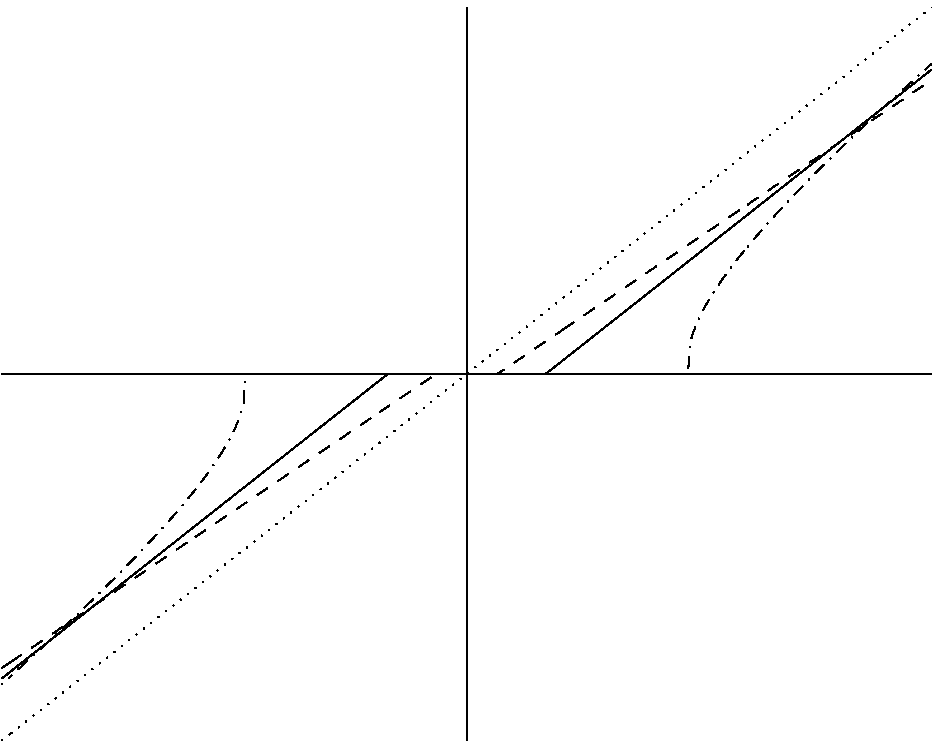
\includegraphics[width=7cm]{fig1401}
%\caption{Cut-off functions for sparse code shrinkage.}
%\end{figure}

%\begin{figure}
%\centering
%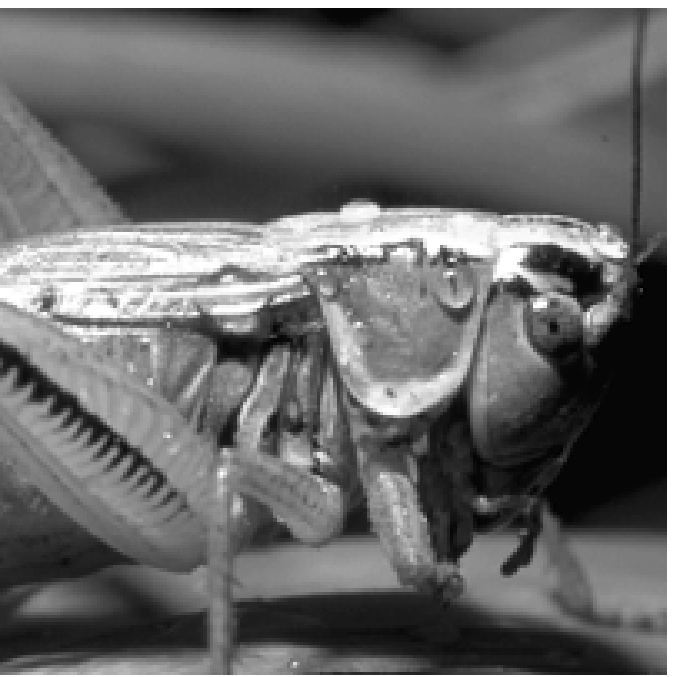
\includegraphics[width=5cm]{fig1907a}
%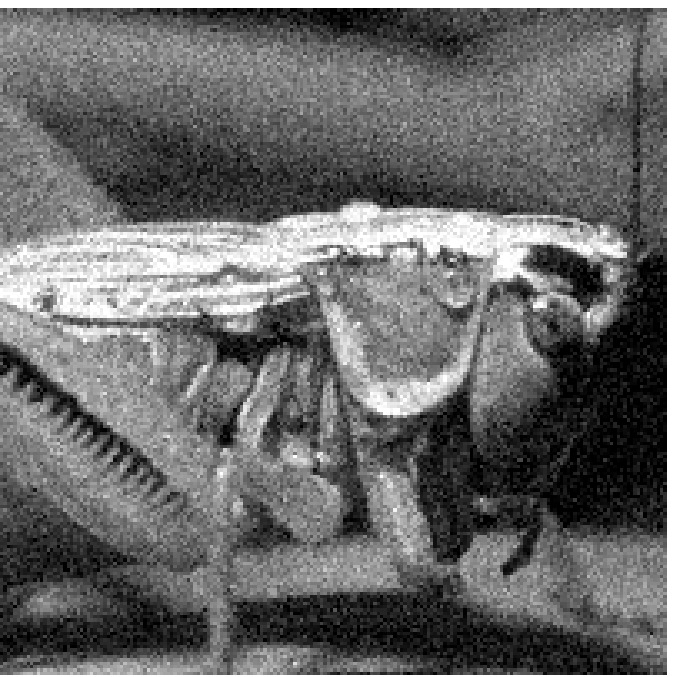
\includegraphics[width=5cm]{fig1907b}\\a \hspace{5cm} b\\
%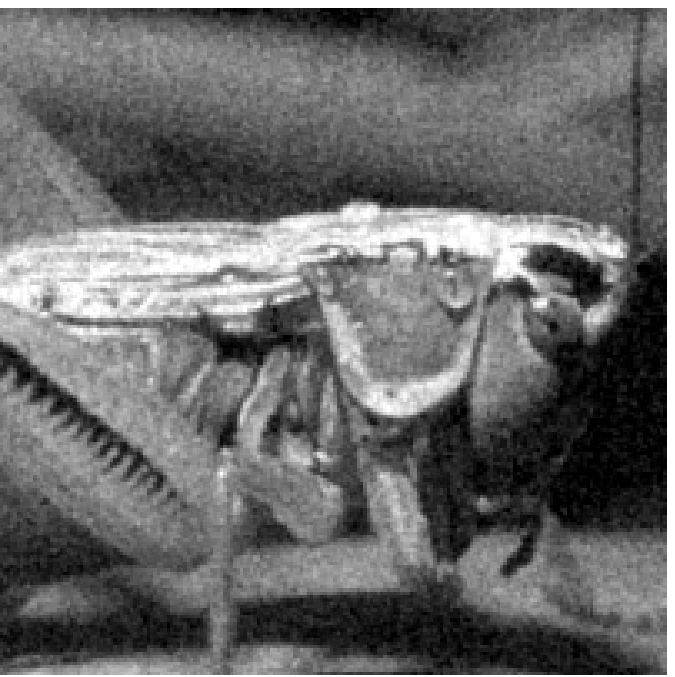
\includegraphics[width=5cm]{fig1907c}
%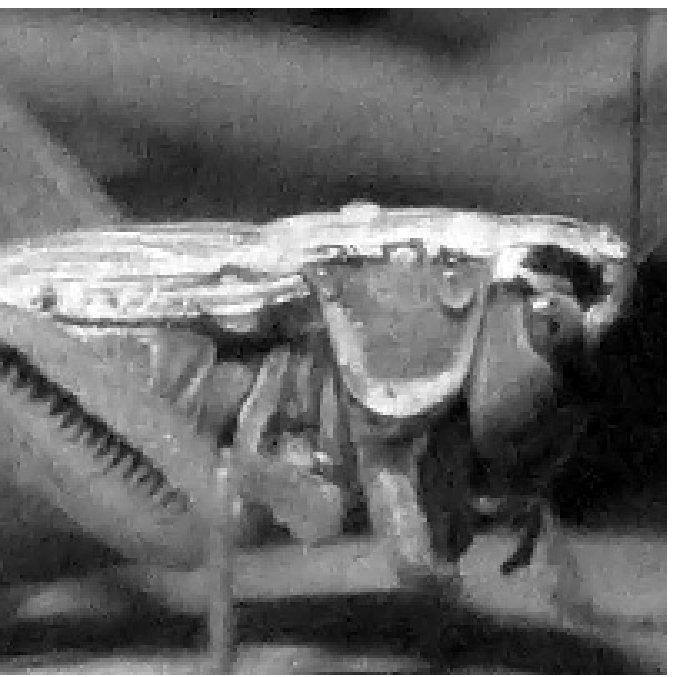
\includegraphics[width=5cm]{fig1907d}\\c \hspace{5cm} d
%\caption{Original noiseless image (a), noisy image (b), wiener
%  filtered image (c), ICA filtered image (d).}
%\end{figure}


%\clearpage
%\item Demo: Source separation from climate data.

\end{enumerate}
\end{document}             % End of document.
